\documentclass{beamer}
\usepackage{color}
\usepackage{bm}
\usepackage{graphicx}
\usepackage{hyperref}
\usepackage{listings}
\beamertemplatenavigationsymbolsempty
\definecolor{mygreen}{rgb}{0,0.6,0}
\definecolor{mymauve}{rgb}{0.58,0,0.82}
\lstset{ %
  backgroundcolor=\color{white},   % choose the background color; you must add \usepackage{color} or \usepackage{xcolor}
  basicstyle=\footnotesize,        % the size of the fonts that are used for the code
  commentstyle=\color{mygreen},    % comment style
  deletekeywords={...},            % if you want to delete keywords from the given language
  extendedchars=true,              % lets you use non-ASCII characters; for 8-bits encodings only, does not work with UTF-8
  frame=single,                    % adds a frame around the code
  keywordstyle=\color{blue},       % keyword style
  language=Python,                 % the language of the code
  rulecolor=\color{black},         % if not set, the frame-color may be changed on line-breaks within not-black text (e.g. comments (green here))
  showspaces=false,                % show spaces everywhere adding particular underscores; it overrides 'showstringspaces'
  showstringspaces=false,          % don't show spaces in strings
  stringstyle=\color{mymauve},     % string literal style
  title=\lstname                   % show the filename of files included with \lstinputlisting; also try caption instead of title
}
\hypersetup{
    colorlinks=true,
    urlcolor=blue
}

\graphicspath{ {./img/} {./charts/} }


\title{Django Under The Hood 2015 Recap}
\author{Adam Johnson - me@adamj.eu}
\date{16 November 2015}

\begin{document}


\maketitle


\begin{frame}[fragile]\frametitle{What is Django Under The Hood?}

    \begin{itemize}
        \item The "newest" Django conference - started last year!
        \item Focus on the internals of Django and contribution
    \end{itemize}

    \begin{center}
        
\includegraphics[width=10cm]{duth-header}
    \end{center}

\end{frame}


\begin{frame}[fragile]\frametitle{What is Django Under The Hood?}

    \begin{itemize}
        \item In Amsterdam, 5th to 7th November
        \item 1.5 days of talks, 1 day of sprints
        \item 300 attendees
    \end{itemize}

    \begin{center}
        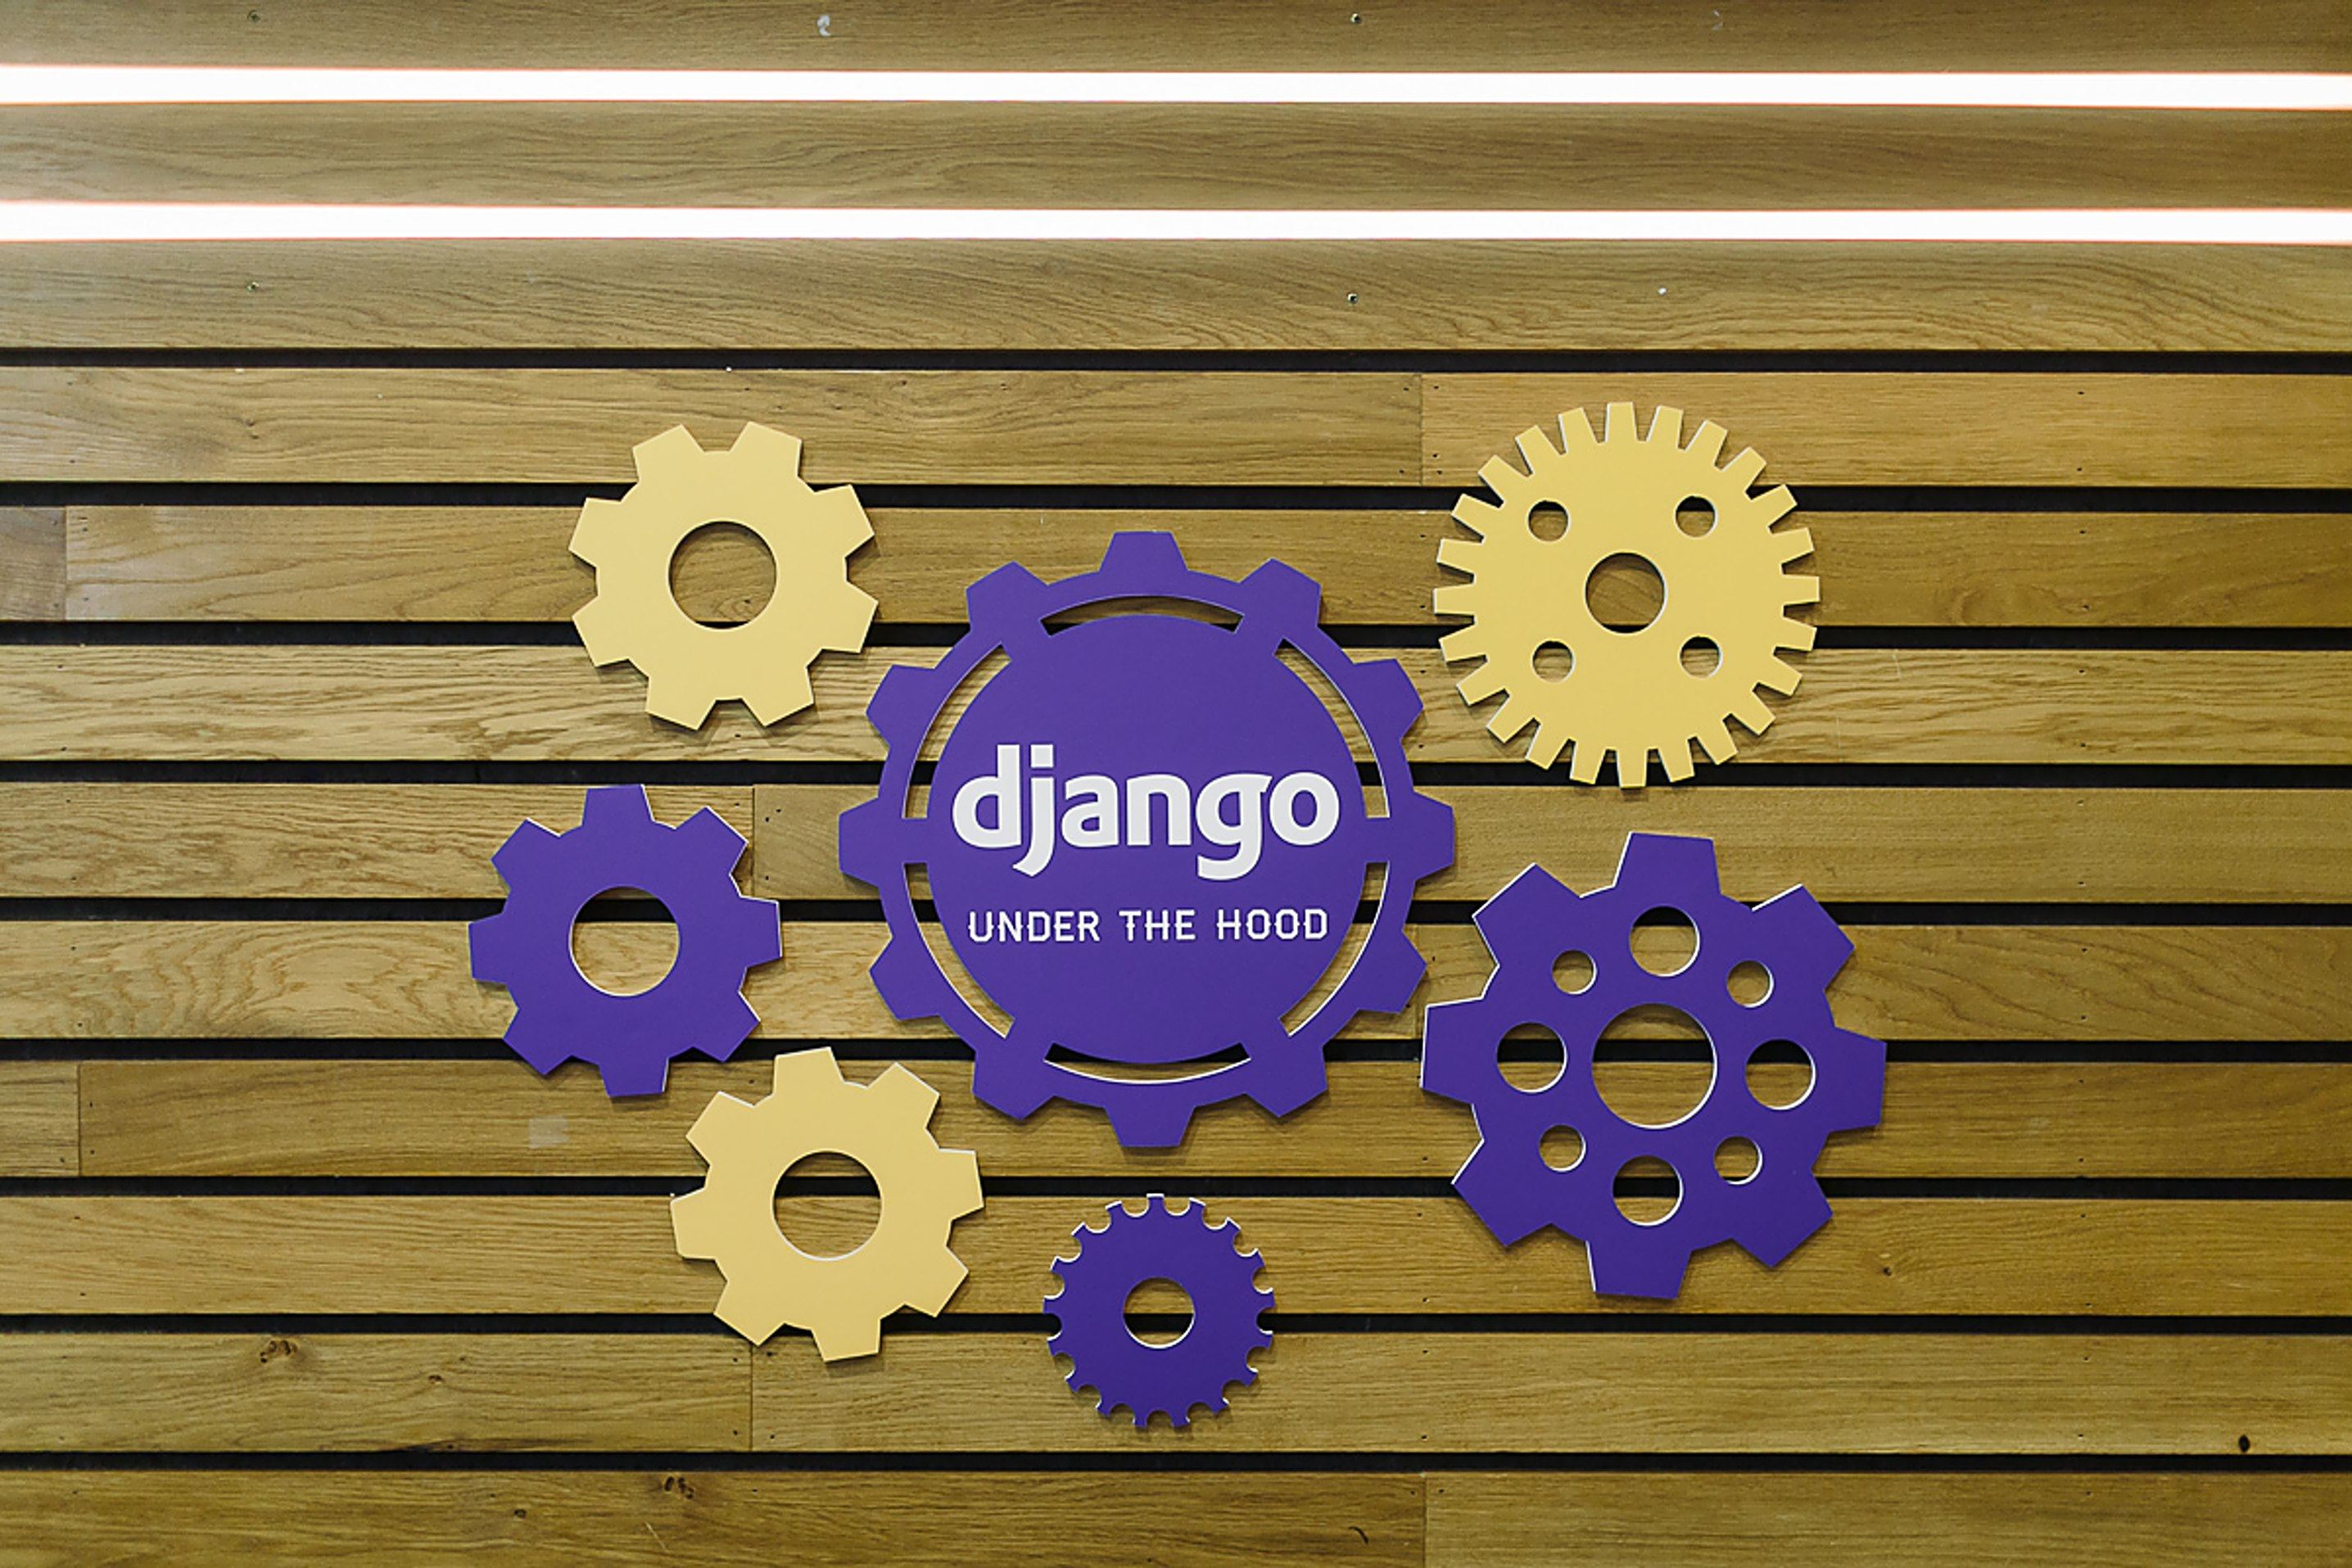
\includegraphics[width=10cm]{duth-cogs}
    \end{center}

\end{frame}


\begin{frame}[fragile]\frametitle{The whole crowd}

    \begin{center}
        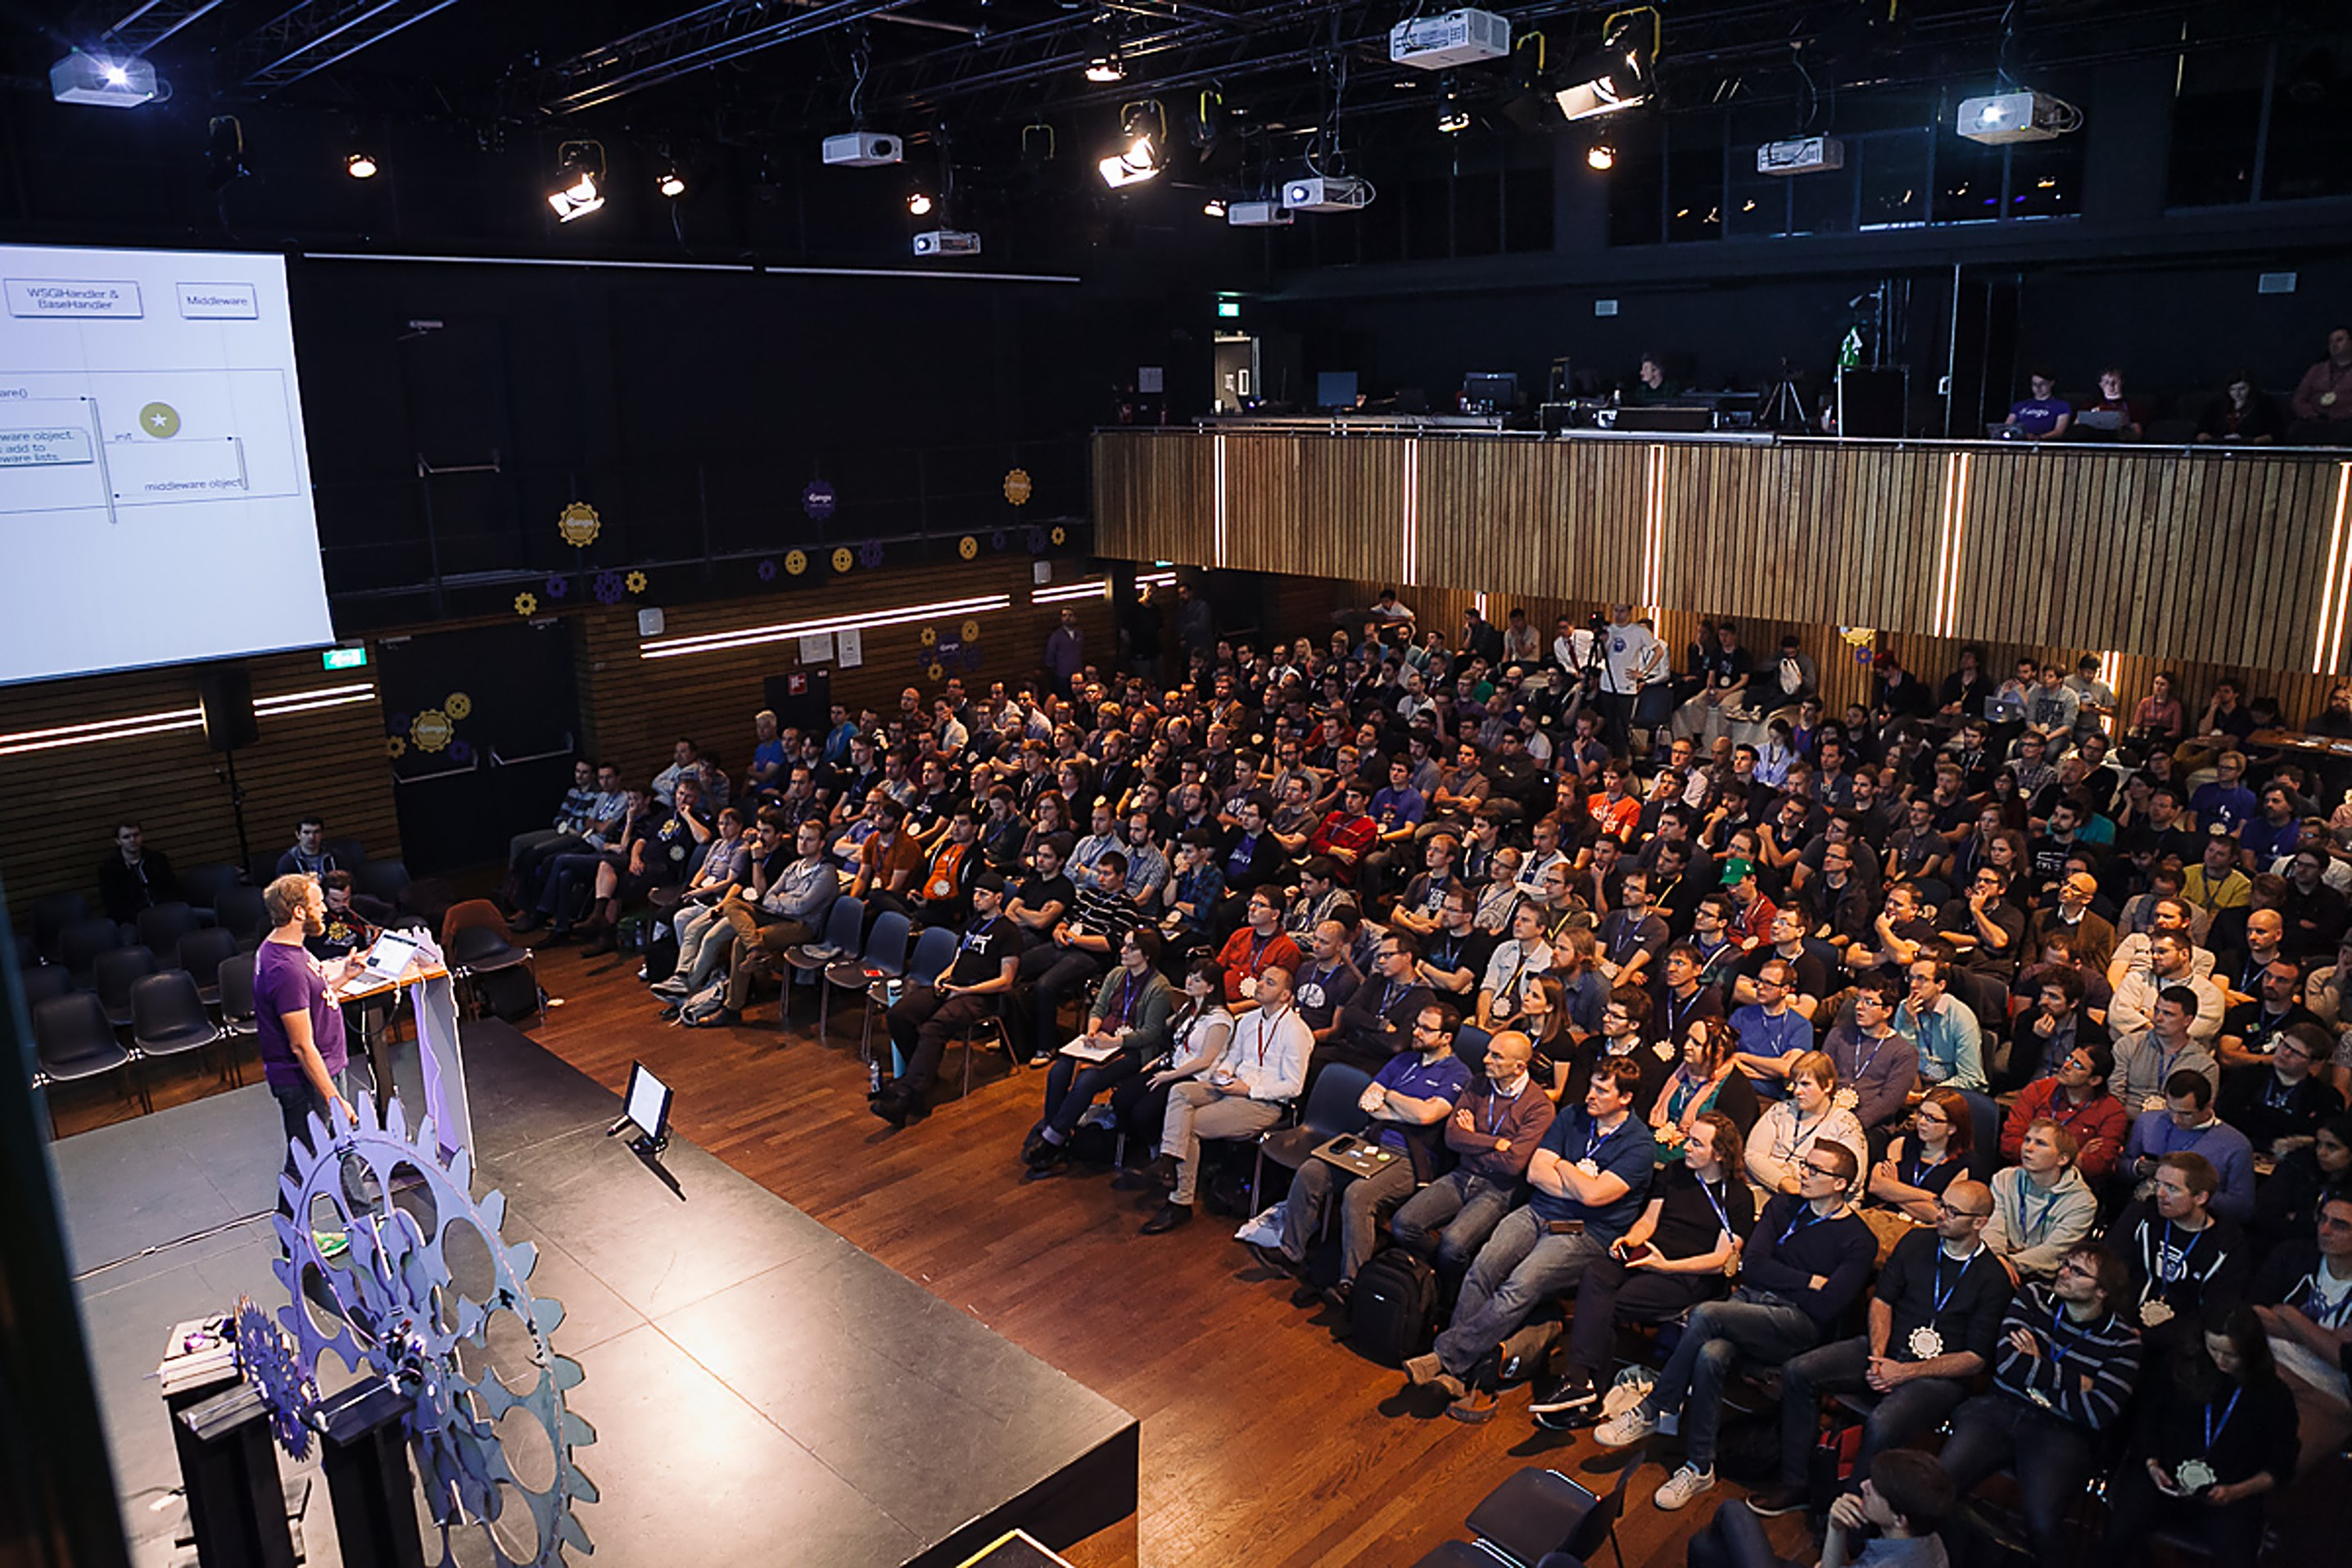
\includegraphics[width=10cm]{duth-attendees}
    \end{center}

\end{frame}


\begin{frame}[fragile]\frametitle{The amazing cog sign}

    \begin{center}
        
\includegraphics[width=10cm]{duth-sign}
    \end{center}

\end{frame}


\begin{frame}[fragile]\frametitle{Team YPlan}

    \begin{center}
        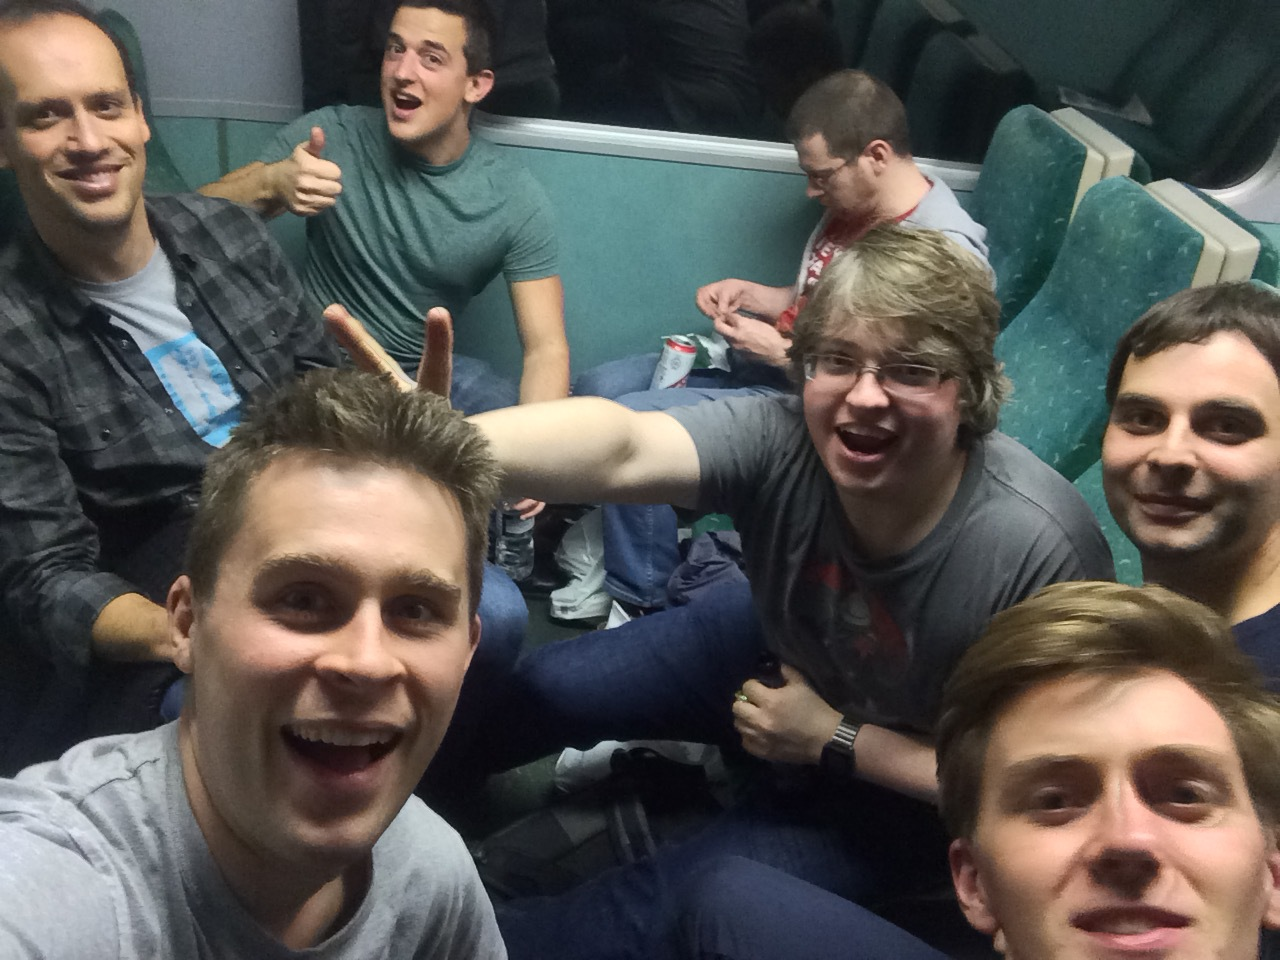
\includegraphics[width=10cm]{yplan-team}
    \end{center}

\end{frame}


\begin{frame}[fragile]\frametitle{Talks}

    \begin{itemize}
        \item 9 talks in a single track, 2 workshops during the sprints
        \item 3 videos online already at \url{opbeat.com/events/duth}
        \item MC'd by Marc Tamlyn
    \end{itemize}

\end{frame}


\begin{frame}[fragile]\frametitle{HTTP in Django - Jacob Kaplan-Moss}

    \begin{center}
        
\includegraphics[width=2cm]{speaker-jacob}
    \end{center}

    \begin{itemize}
        \item One of the originators of Django
        \item Covered how Django interfaces with your \texttt{WSGI} web server, converts requests into \texttt{WSGIRequest} objects, passes them through your middleware and views, then takes the \texttt{HTTPResponse} you return and passes that back to WSGI
        \item Covered the history too, including the invention of WSGI
    \end{itemize}

\end{frame}


\begin{frame}[fragile]\frametitle{Django Admin - Ola Sitarska}

    \begin{center}
        
\includegraphics[width=2cm]{speaker-ola}
    \end{center}

    \begin{itemize}
        \item One of the DUTH organizers
        \item Covered how the Admin works, the interaction between the \texttt{ModelAdmin} class and \texttt{ChangeList}, as well as pointing out some places it needs improvement
    \end{itemize}

\end{frame}


\begin{frame}[fragile]\frametitle{Django CMS & ORM - Iacopo Spalletti}

    \begin{center}
        
\includegraphics[width=2cm]{speaker-iacopo}
    \end{center}

    \begin{itemize}
        \item Invited as a creator of a large third party app
        \item Explained how Django CMS integrates with Django, how its plugin infrastructure works, and some of the pain points/hacks that are necessary
    \end{itemize}

\end{frame}


\begin{frame}[fragile]\frametitle{Keynote - Russell Keith-Maggee}

    \begin{center}
        
\includegraphics[width=2cm]{speaker-russ}
    \end{center}

    \begin{itemize}
        \item President at Django Software Foundation
        \item Walked through the commit history of Django, pointing out major changes and funny messages - gave a good background to why some things are the way they are
    \end{itemize}

\end{frame}


\begin{frame}[fragile]\frametitle{Twisted \& Django - Amber Brown}

    \begin{center}
        
\includegraphics[width=2cm]{speaker-amber}
    \end{center}

    \begin{itemize}
        \item Release Manager for Twisted
        \item Talked on how Twisted works to provide asynchronous capabilities in Python, and gave a PoC integration of Django and with Twisted
        \item The future of django may be asynchronous - see \url{github.com/andrewgodwin/channels}
    \end{itemize}

\end{frame}


\begin{frame}[fragile]\frametitle{Static files in Django - James Aylett}

    \begin{center}
        
\includegraphics[width=2cm]{speaker-james}
    \end{center}

    \begin{itemize}
        \item Long time Django developer
        \item Covered how static files work in django, the difference between 'static' and 'staticfiles', and a lot of the crusty tickets to do with static file handling.
    \end{itemize}

\end{frame}


\begin{frame}[fragile]\frametitle{Django Security - Florian Apolloner}

    \begin{center}
        
\includegraphics[width=2cm]{speaker-florian}
    \end{center}

    \begin{itemize}
        \item Head of Django Security
        \item Covered Django's security policies, existing security features and the future of security
    \end{itemize}

\end{frame}


\begin{frame}[fragile]\frametitle{Documentation Systems - Eric Holscher}

    \begin{center}
        
\includegraphics[width=2cm]{speaker-eric}
    \end{center}

    \begin{itemize}
        \item Creator of Read The Docs
        \item Covered how Sphinx works internally, and given this, how it can be integrated with other syntaxes such as Markdown
    \end{itemize}

\end{frame}


\begin{frame}[fragile]\frametitle{The Sprints!}

    \begin{center}
        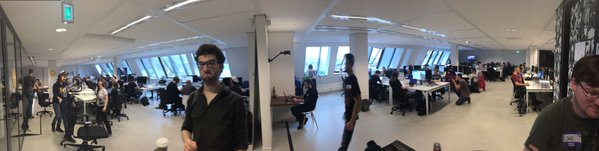
\includegraphics[width=10cm]{duth-sprints-panorama}
    \end{center}

    \begin{itemize}
        \item Amazing venue thanks to Travelbird
        \item Over 100 people getting involved with improving Django and related packages
    \end{itemize}

\end{frame}


\begin{frame}[fragile]\frametitle{The Sprints!}

    \begin{center}
        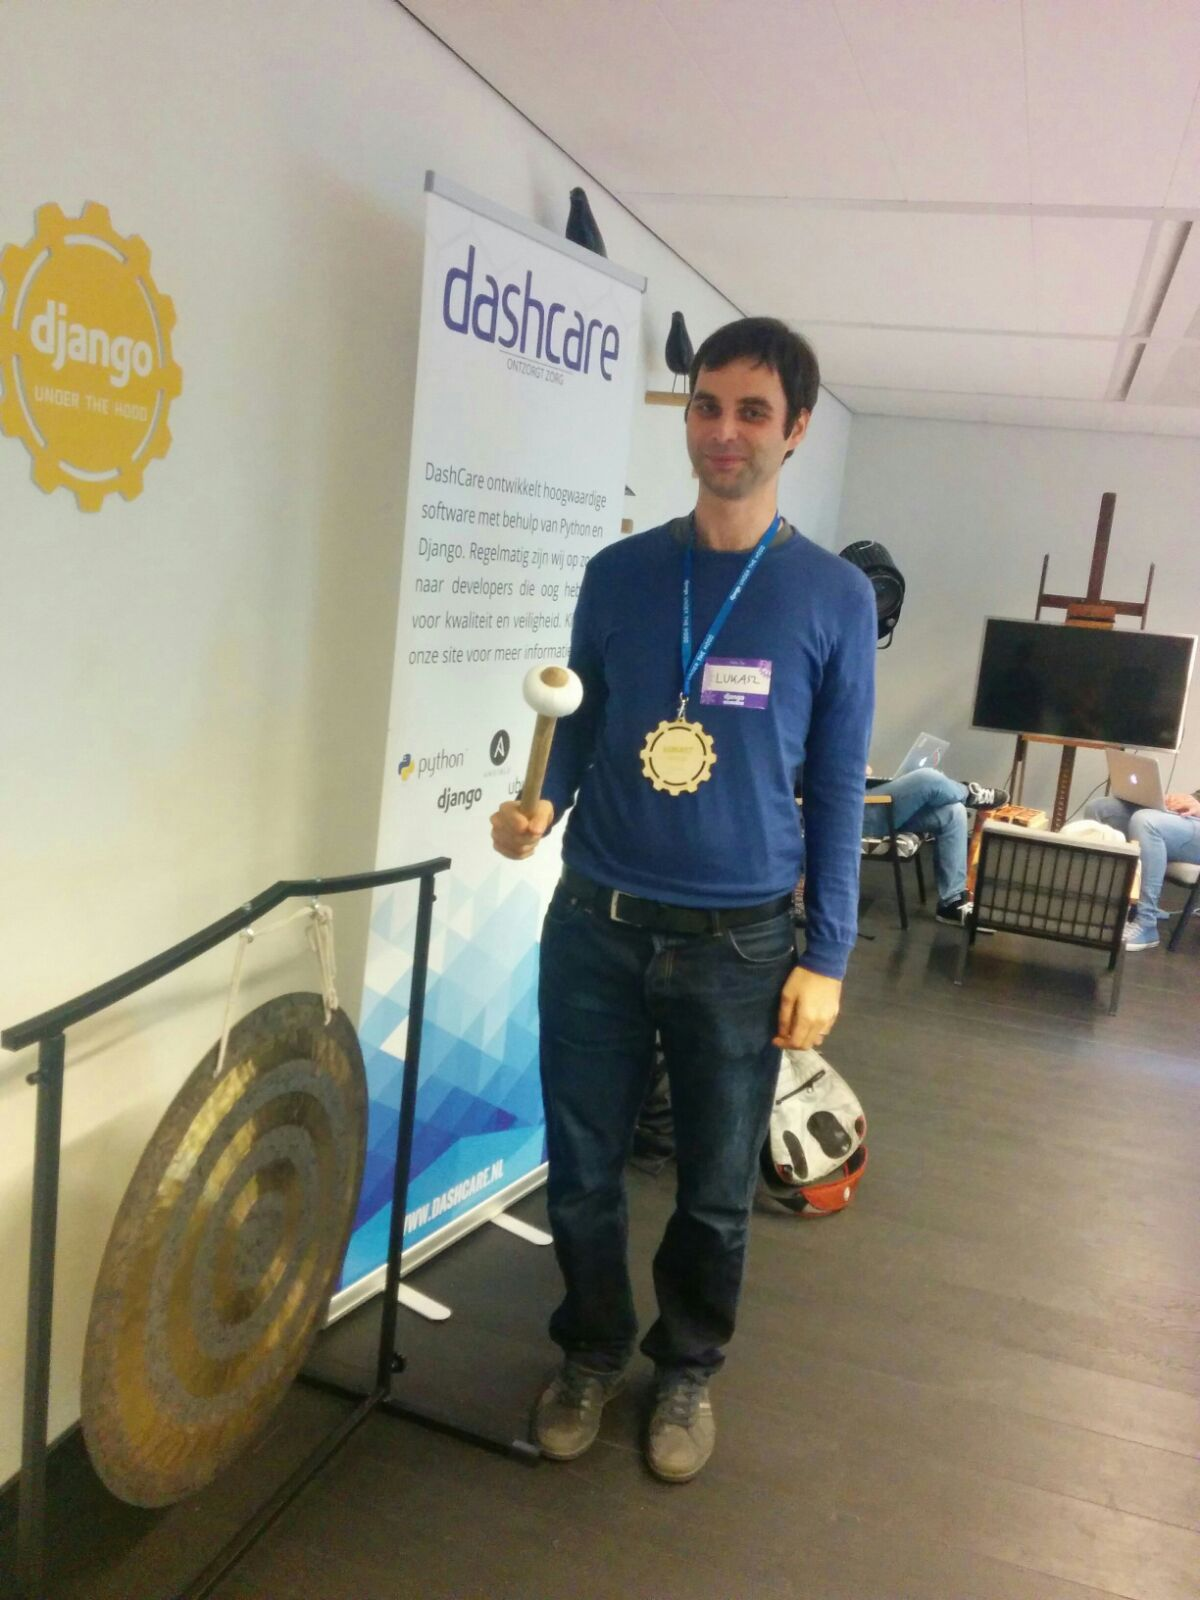
\includegraphics[width=5cm]{duth-sprints-lukasz-gong}
    \end{center}

    \begin{itemize}
        \item Every commit/issue - bang the gong! The whole room cheers!
    \end{itemize}

\end{frame}


\begin{frame}[fragile]\frametitle{The End}

    \begin{center}
        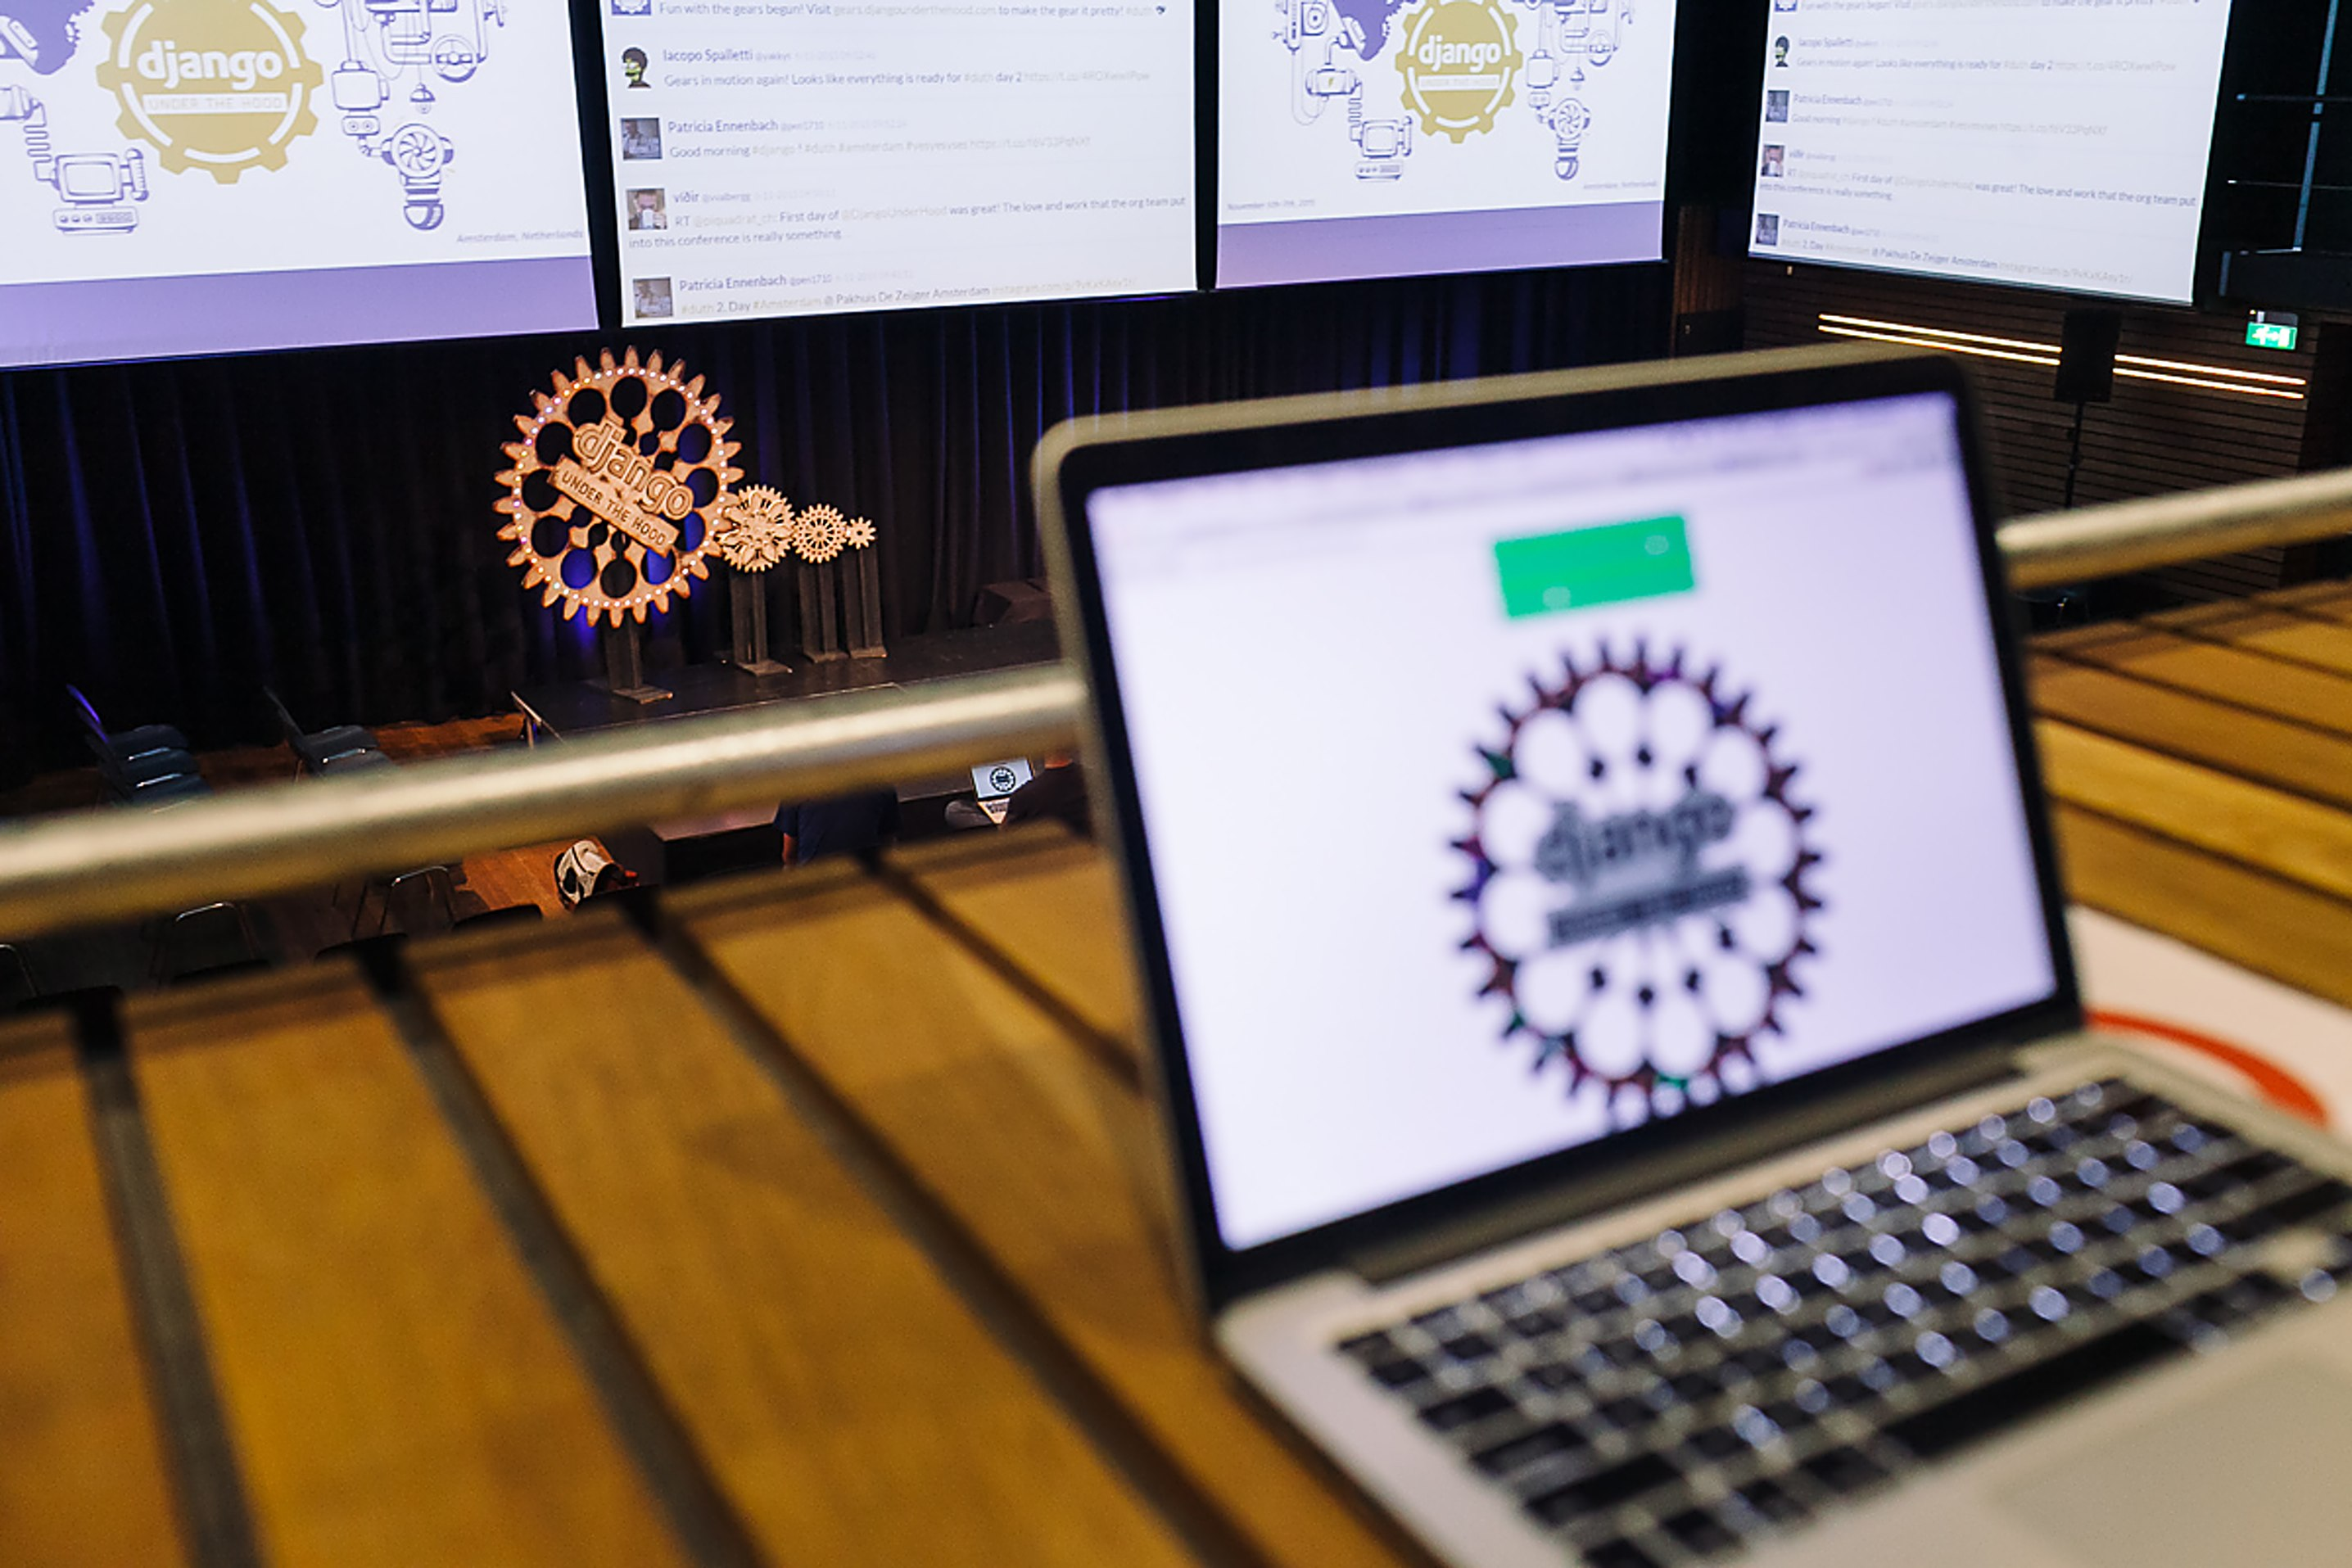
\includegraphics[width=8cm]{duth-the-end}
    \end{center}

    \begin{itemize}
        \item Website: \url{djangounderthehood.com}
        \item Talk videos: \url{opbeat.com/events/duth/}
        \item My blog: \url{adamj.eu/tech/}
    \end{itemize}

\end{frame}


\end{document}
